\chapter{Model}
\label{chapter:model}

\minitoc[n] % minitoc without title

\section{Introduction}

  \subsection{Why Model the Evolution of Cooperation}

    In this chapter, our approach is one of modeling to study the evolution of cooperation. As in most fields in science, modeling is an obvious approach to study problems that cannot be comprehended by simply observing the physical world. Thus models are now commonly accepted in the realm of evolutionary biology, even if this may not have been the case for a long period of time~\cite{Shou2015}; the next Subsection will be devoted to reviewing the different modeling techniques used in evolutionary biology and what they brought more precisely on the evolution of cooperation. In this present Subsection however, we are interested in quickly reviewing the more empirical study of evolutionary biology as to justify the need to use models in our case. 

    Everything that we contemplate now is the consequence of thousands of millions years of evolution; earliest appearance life is dated to $4000$ millions years ago and a little more than $2000$ millions for the eukaryotes. The time scales involved in the evolutionary process thus are such that we cannot directly observe evolution but rather try to figure for the most part how it could take place. This means that we are mostly left with evidences from the past. To that end, most discoveries come from paleontologists and the analysis of bones from past periods. A copious amount of work in particular has been dedicated to studying the past social life of our hominin ancestors. For example, paleontological records allow to have a better understanding of the diet of early hominins. More importantly, those records reveal a strong correlation in our ancestors between the switch to a more energy-rich diet (e.g. meat) and the increase in the brain size of these ancestors~\cite{Aiello1995, Wrangham1999}. 

    This would then suggest a coevolution between the transition to a rich diet and the appearance of social behaviours (which require higher brain functions~\cite{Dunbar2007, Isler2012}). Theories and how exactly this transition shaped cooperation are diverse~\cite{Pontze2012}. Some think that this new diet could allow to adopt more diverse and more efficient hunting and scavenging techniques. Indeed, a richer diet would be necessary to develop the locomotive and cognitive skills necessary for both of these activities~\cite{Aiello1995, Bramble2004}. Some others believe a shift in climatic conditions led to the early hominins to rely more on underground storage organs. While this type of food is rich and available even under arid climate, its harvesting is difficult. This drove the selection for the capacity to share food among individuals, thus leading to cooperation~\cite{O'Connell2002}. Some even believe this led to cooking this food which created a physical location where individuals would meet and thus create social dynamics~\cite{Wrangham1999, Wrangham2009}. Therefore, those paleontologic evidence can be used to hypothesize on the ecological conditions and the selective pressures that applied and could shape the evolution of cooperation.

    But theories can also be formulated by looking at the present rather than the past. In fact, most of the empirical work in studying the evolution of cooperation was achieved by directly observing animal behaviours (mostly non humans). While understanding the evolution of cooperation in any social animal is interesting on its own, it is also believed that it could help understand mankind could achieve such high levels of sociality. For example, convincing links have been made between the evolution of cooperation in humans and in social carnivores~\cite{Schaller1968, Smith2012} (which is also a strong argument in favor of the correlation between a transition to a rich diet comprised of meat and the evolution of cooperation). More generally, ethology (i.e. the study of animal behaviour), helps theorize the mechanisms which shaped the evolution of cooperation.

    For example, as previously explained in the Introduction, most research on the evolution of cooperation has been centered on studying the evolution of altruism. And as such, much research focus on finding evidence of kin selection in animals~\cite{Bourke2014}. To that end, a copious amount of work has been dedicated to the evolution of eusociality. Only $2\%$ of insect species are eusocial but they represent most of the insect biomass~\cite{Wilson2008}, the most obvious of representatives coming from the hymenoptera order (e.g. ants, bees or wasps). Those insects are known to exhibit astonishing levels of altruisms which have been explained by the inclusive fitness theory~\cite{Bourke2011, Wilson2008}. The most convincing example is the presence of the reproductive division of labour. This means that only a certain "caste" of individuals will have the right to reproduce, which are called queens (or kings)~\cite{Wilson1990}. As we mentionned while defining altruism, this seems to directly contradict the process of evolution where individuals are selected for their capacity to reproduce. However, it has been observed that colonies of eusocial individuals are composed of strongly related organisms. In particular, all members of the colony are offsprings of a single individual (i.e. the queen). This can explain how a "genetic trait" that encourage individuals to give up on their reproductive rights can spread in the population (because it helps spread the genes of genotypically similar individuals)~\cite{Queller1998}.

    % Naked mole-rat ?

    But kin selection has also been investigated and successfully revealed in vertebrates. In particular, it has been shown that in most cooperative species of birds and mammals, social groups are small and composed of dominants breeders and their relatives~\cite{Dugatkin1997, Clutton-Brock2002}. This explains the differences in breeding (what is called reproductive skew) between individuals of the same group and the rearing of youngs by individuals which are not their parents. The evolution of such highly cooperative behaviours can be explained by kin selection in the same way that reproductive division of labour exists in eusocial insects~\cite{Bourke2011}. However, where kin selection was mandatory to explain the evolution of such altruism in eusociality, the importance of kin selection among vertebrates is much more debatable~\cite{Griffin2003, Clutton-Brock2002}.

    In particular, ethology studies in verterbrates have in the past decades been focused on the importance of direct fitness benefits in cooperation. Progress in this direction are difficult because most of observations of cooperative actions in verterbrates are likely to result from a combination of both indirect and direct benefits~\cite{Clutton-Brock2009}. However, while rare in comparison to cooperation inside strongly related groups, the presence of cooperation between unrelated individuals must be explained by direct benefits to fitness. In particular, the spotted hyenas are known to cooperate with kin and non-kin alike to achieve collective hunting and defense against other predators~\ref{Drea2009a, Smith2010, Smith2012}. Thanks to field work on cooperative vertebrates, different theories on how could direct benefits take place in cooperative interactions have been proposed~\cite{Clutton-Brock2002}. First, cooperative breeding could be explained by group augmentation. This means that individuals have a direct benefit in increasing group size: better protection against predators, more efficient catching and defense of food and the rearing of youngs~\cite{Packer2001}. Secondly, a lot of cooperative interactions could be explained by mutual benefits (i.e. intraspecific mutualism). Primates are known to engage in mutual grooming and birds can build communal nests which directly benefit every participants. Obviously collective hunting can profit to every individuals by increasing the product of the hunt and decreasing the risk (both in term of being wounded by the prey and not being able to catch it)~\cite{Scheel1991}. Finally, cooperation can be enforced through coercion where non-cooperative individuals could suffer punishment or eviction from the group. Reciprocity~\cite{Trivers1971}, where individuals will cooperate with partners with which they previously interacted has often been proposed to explain cooperation between non-kin. However at the moment, there is no sufficient evidence that this type of behaviour occurs in other vertebrates than humans~\cite{Hammerstein2003, Clutton-Brock2009, André2014}.

    % Je mentionne peu les primates ici. Ca serait bien d'en parler très rapidement (après tout on apprend pas beaucoup de choses vraiment différentes (voir même moins qu'avec les hyènes d'après Drea2009a))

    While different in the manner they are done, studies on cooperation in humans also obviously exist. Economists have been focused on human altruism and have produced experiments to display the existence of profound evidence of altruistic cooperation between non-kind~\cite{Fehr2002, Fehr2003}. Because kin selection only cannot be involved here, altruism in human societies is best explained by a pattern of rewards, reputation and punishment. In particular, they showed the importance of strong reciprocity between humans. While altruistic reciprocator will reward and punish individuals if they have a long-term interest~\cite{Trivers1971}, strong reciprocators will do so anyway (i.e. in a stricly altruistic way). Fehr and Fischbacher~\cite{Fehr2003} argue that the evolution of human altruism cannot be only explained by gene-based evolutionary theory alone and advocate for of gene-culture coevolution.

    Because the subject of this dissertation is on the mechanisms of coordination involved in mutualistic actions, it is interesting also to note that some have also been interested in that aspect of human cooperation. For example, Michael Alvard has studied societies of traditional whale hunters of Lamalera in Indonesia~\cite{Alvard2001, Alvard2003}. He has been interested in showing that in that case there is no relation between strong kinship and an increase in cooperation in these societies. Alvard thus argues for more mutualistic explanations for the evolution of coordinated actions. Moreoever, other studies have also been focused on the mechanisms with which humans coordinate to solve cooperation problems. For example, Bullinger and colleagues~\cite{Bullinger2011, Duguid2014}, have studied how exactly chimpanzees and human childs coordinate in a stag hunt type of game. They have mostly focused on the role of communication and leadership strategies between individuals.

    Lastly, there is in particular conditions the possibility to direclty "watch" evolution happens. This is done in organism where evolution is a fast process: microorganisms~\cite{Elena2003}. For example, Richard Lenski is known for his "Long-Term Evolution Experiment" on Escherichia coli~\cite{Fox2015}. This experiment began in 1988, when Lenski set up $12$ populations of the same genotype of E. coli and observed their evolution since then. But more generally, bacteria are known to display acts of behaviours that can be caracterized as cooperative~\cite{West2006}. For example, we previously talked about the public goods game to which bacteria participate when they produce nutrients which can be enjoyed by any other bacteria in the vicinity~\cite{Harrison2013}. Some microorganisms are known to behave altruistically. For example, some cells of the slime mould Dictyostelium discoideum sacrifice themselves so that other cells can become spores and thus spread their genes~\cite{Strassmann2000}. Thus microorganisms have been used to again validate kin selection and kin discrimination~\cite{West2006}. In particular, while green beard mechanisms are though to be rare, D. discoideum have an exemple of this mechanisms, where one gene allows individuals to adhere to each other to cooperatively form fruiting bodies~\cite{Queller2003}. But evidence of direct benefits between microorganisms have also been revealed. Mutualism (i.e. interspecific coopration) is frequent between microorganisms where it can provide direct by-product benefits. Evidence of punishing behaviours have also been shown in mutualism between plants and bacteria, like between leguminous plants and the rhizobial bacteria~\cite{Kiers2003}. The bacteria fix $N_{2}$ at a cost which is supplied to the plant. The plant enforces cooperation by decreasing the supply of $O_{2}$ to the bacteria if they defect. To conclude, it also interesting to note that there are pratical medical applications for studying the evolution of cooperation in microorganisms as there exists a correlation between cooperation and the virulence of bacteria strains~\cite{Foster2005}.


    In conclusion, empirical studies on the evolution of cooperation exist and are widespread. However, they have been a larger focus on studying the evolution of altruism and veryfing kin selection related theories. And even when mutualistic actions are considered, they rarely inform on the mechanistic constraints involved in the evolution of cooperative actions: proximate causes are hard to finely study when you can only observe the ultimate results of such a long process. In comparison, in the particular case of microorganisms, microbiologists are often concerned with proximate explanations of cooperation~\cite{West2006}. However, they do not unfortunately offer the wide range of cooperative behaviours with which bigger organisms are concerned.

    % Parler de ce que dit Smith sur protection against predators ?
    % Man the hunted

    % Phylogénétique ?

  \subsection{Classical Modeling in Biology}

    As previously said, it is now classical in evolutionary biology to model the evolution of cooperation (among any evolutionary trait). Models are numerous and a lot of different frameworks have been proposed to classify cooperative actions~\cite{Dugatkin2002, Sachs2004, Lehmann2006}. To that end, purely mathematical models dominate the field~\cite{Servedio2014}. In particular, \emph{population genetics} form a large part of the litterature in evolutionary biology. This field was mostly created by the works of Ronald Fisher, J.B.S. Haldane and Sewal Wright. Fisher was the first to link mendelian inheritance (i.e. the theory on the inheritance of biological traits) with mathematical models of natural selection in his book \textit{The Genetical Theory of Natural Selection}~\cite{Fisher1930}. Population genetics is concerned with studying the change in frequency of alleles of particular locus in the genotype across generations. Various studies used population genetics to approach evolutionary problems as diverse as 
    
    -> Parler de kin selection ici
    -> Good for ultimate explanations

    % Reprendre la partie sur population genetics

    In comparison to the genetic modeling of evolution with population genetics, another type of models were created to focus on a phenotypic view of evolutionary biology: \emph{evolutionary game theory} (EGT). Game theory was originally conceive by the mathematician John von Neumann as a way to determine the optimal strategies in a contest between several (usually two) "players". Given what is called a payoff matrix, each player can expect a certain payoff depending on her strategy and those of the other players. In this framework, players are expected to be rational and follow this optimal strategies. One of the most important concepts of game theory is the \emph{Nash equilibrium}~\cite{Nash1950}. Under such equilibrium, no player can benefit from changing her strategy if the other players keep their strategy. This framework was first adapted to darwinian evolution by John Maynard Smith and George Price under the name of evolutionary game theory~\cite{MaynardSmith1973}. Under this name is the idea that, rather having players choosing a strategy based on a rational decision, individuals in a population simply play a strategy based on their phenotypes. Therefore, this strategy is now inherited and not chosen and we want to study the evolutionary perspective of the different strategies. To that goal, the payoff of the evolutionary game new corresponds to the fitness value of each strategy. The basic principle of evolutionary game theory is to consider a population of individuals all playing the same strategy. We then imagine the appearance of a rare mutant who plays a different strategy and study the evolutionary dynamics of these two strategies. If the strategy of the mutant has a higher fitness than that of the initial population (called the \emph{resident strategy}), then it will invade the population and may replace the resident strategy. Otherwise, the mutant strategy will be selected against and disappear. If this resident strategy is stable against any mutant strategy, then we say this strategy is evolutionarily stable (ESS)~\cite{MaynardSmith1973}. Interestingly, all ESS are Nash equilibria (but the opposite may not be true).

    One of the main feature of evolutionary game theory in comparison to population genetics is that it takes into account the influence of one individual's behaviour on the fitness of others. More precisely, the fitness of one individual will depend on the proportions and behaviours of other individuals in the population, which is know as \emph{frequency-dependent selection}. As such, EGT is convenient for taking into consideration the ecological features of particular evolutionary phenomenon~\cite{Hammerstein1994}. As it models interactions of cooperation and conflicts, it has been of great interest for the study of the evolution of social behaviours~\cite{Bshary2015}. One such famous study was that of reciprocity in the \emph{Iterated Prisoner's Dilemma}~\cite{Axelrod1984}. The prisoner's dilemma was already a very famous game theoretic model (of which you can find Axelrod & Hamilton's payoff matrix in Table~\ref{table:payoffIPD}) but Axelrod & Hamilton proposed that individuals play an iterated version of this game. In summary, two individuals who play an interaction have a probability to meet again. They show that, under those circumstances, the evolutionary stable strategy is one called \emph{Tit for Tat} (TFT). Under this strategy an individual always cooperate when meeting an opponent for the first time. She then always copy the opponent's last move which means that (1) she retaliates and (2) she does not hold grudges. This strategy was thus presented as a theoretical example of the success of reciprocity~\cite{Trivers1971}. More generally, a large body of work has been focused again on the evolution of altruism against the appearance of free-riders (defectors) in EGT thanks to the prisoner's dilemma~\cite{RequejoMartinez2013}.


    \begin{table}[ht]
    \centering
      \caption{\textbf{Payoff matrix of the prisoner's dilemma.}}
      \begin{tabular}{l|c|c}
        & Cooperation & Defection
        \hline
        Cooperation & 3,3 & 0,5
        \hline
        Defection & 5,0 & 1,1
        \hline
      \end{tabular}
      \begin{flushleft} The strategy of player A (resp. player B) is symbolized by each row (resp. column). The payoffs to both players are shown such that the payoff of player A (resp. player B) is on the left (resp. right). 
      \end{flushleft}
    \label{table:payoffIPD}
    \end{table}


    As previously said here we are interested in the problem of coordination. For this type of social interaction, as for actually most of social interactions, the prisoner's dilemma is not sufficient to model the evolutionary dynamics of cooperation~\cite{Alvard2002, Skyrms2004}. This is why there has been some interest on another model: the stag hunt~\cite{Skyrms2004, RequejoMartinez2013}. We will not go in detail here in describing this game as it was already done (although briefly) in the Introduction. What is important to know is that the major difference with the prisoner's dilemma is the presence of a second ESS which is the cooperative equilibrium. Thus the emphasis of this game is not on the risk of the invasion of a population of cooperators by free-riders (as cooperation is evolutionarily stable) but on the transition from the solitary equilibrium to the cooperative one. In his original book, Skyrms used this framework to study how some hypothesis on how to solve this particular problem. Mainly, he studied the influence of location, signaling and partner choice~\cite{Skyrms2004}. While the literature on this coordination game is much smaller than that on the prisoner's dilemma, still there has been very interesting work on this subject~\cite{Santos2005, Pacheco2009, Iyer2016}.

    But in classical EGT, strategies are discrete and constitute a finite list. This is a particular side of EGT which is focused on what are called matrix games. In comparison, most traits in evolutionary ecology take their values in a continuous domain. We can for exemple think about the size, flowering rate or the investment and allocation of resources~\cite{McGill2007}. In order to study the evolutionary dynamics of those traits, a continuous version of EGT rose under the name of adaptive dynamics (or sometimes simply continuous-trait game theory). This modeling technique can be seen as a way to combine population genetics, by studying the rate of change of a population's strategy, and EGT, by using the concept of frequency-dependent selection~\cite{Geritz1998, McGill2007}. More precisely, adaptive dynamics extends on the main notion of EGT: the evolutionary stable strategies. In particular, the concept of ESS as it exists in EGT lacks any knowledge about the convergence of a given strategy. To put it more simply, we know that a strategy which is ESS will not be invaded by any mutant strategy once it has spread in the population. Yet, we do not know if this strategy will actually become established. This later dynamic is defined by \emph{convergence stability}, a notion which defines the fact that a strategy, thanks to multiple small evolutionary steps, will be able to appear. Both concepts of evolutionary stability and convergence stability do not always come together~\cite{Eshel1981, Eshel1983}. Behind convergence stability is the idea that the shape of the fitness landscape changes as the population's strategy is changing. From this it stems that it may be impossible to evolve an ESS that may be a maximum of fitness.

    Adaptive dynamics have been really useful in understanding complex phenomenons that may not have been studied under classical game theoretical framework. First, they introduced the concept of "branching points". These occurs when a strategy is convergence stable but not evolutionarily stable~\cite{Geritz1998}. This happens because this strategy acts as evolutionary attractor from afar but, because the fitness landscape changes as the resident strategy changes, this strategy may be a fitness minimum (and thus not ESS). These are called branching points because two different evolving population may coexist and evolve separately. Branching points have thus been used to model the evolution of speciation~\cite{Geritz2004}. Coevolution has also been widely studied in this field, thanks in particular to the modeling of frequency-dependence. For example, the competitive coevolution of predators and preys, and how branching points influence the apperance of niches in these systems~\cite{Bowers2003}. But cooperative coevolution has also been studied. Namely, the evolution of mutualism (i.e. interspecific mutualism). The mechanisms that could allow its evolutionary stability against cheaters has thus been studied~\cite{Ferriere2002, McGill2005}. (TD: Phrasing bien pourri là) Finally, it goes without surprise that altruism has had its fair share of research under adaptive dynamics. Most notably, the ecological aspect of adaptive dynamics (as in game theory in general) allowed to studied how dispersal could be a prominent mechanism to decrease kin competition and thus allow kin selection to effectively enable the evolution of altruism~\cite{LeGalliard2003, LeGalliard2005}.

    % Main criticism But the thing is beyond an invasion threshold 
    % -> Mentionner les différents types de jeux ? (coordination games, PD etc... (ya un papier là-dessus))
    

  % Parler plutôt de Computational Biology ? J'aime bien l'idée de parler de techniques de modélisations particulières qui s'inscrivent finalement dans cette opposition plus générale de Classical VS Computational
  \subsection{Individual-Based Modeling and Evolutionary Robotics}

    The different modeling techniques presented before are sometimes named "classical models"~\cite{Huston1988, Adami2014} and this how we will refer to them in this manuscript. It is important to understand this is not used in a derogatory fashion to distinguish between the old and the new. This is rather a way to discriminate between the classical models, which are usually purely mathematical analytical models and which have been classical in evolutionary biology, and a range of models which were born thanks to the easier and easier access to computational power. This allowed to approach biological problems in a very different way and, some would argue, to go beyond what is possible with purely mathematical modeling~\cite{Adami2012}. More generally, computational models allow for the addition of stochastic effects, which are essential to the modeling of most of evolutionary mechanisms (e.g. how population dynamics happen in finite populations) and thus are an important addition to classical models. However, it is important to note that sometimes the line between classical and computational models can sometimes be not so easy to draw and there is a real scientific interest in trying to get the best of both worlds~\cite{Wilson1998}.

    One such computational method which has had a big influence on behavioral ecology is \emph{individual-based modeling}\footnote{It is important to note that the term \emph{agent-based modeling} can often be found in the litterature in lieu of individual-based modeling. Both names refer to the same technique and can be used interchangeably. While individual-based modeling (IBM) seems to be found more often in biological applications~\cite{Grimm2005}, no real consensus exist on which term to use. We choose to use the latter throughout this manuscript.}.


    \begin{itemize}
      \item{Review of people that are doing the same thing in IBM (Avida, ER etc...)}
    \end{itemize}







































%%% ----------------------- ARTICLE 1 ----------------------- 
\section{To Cooperate or not to Cooperate: why Behavioural Mechanisms Matter}
  \subsection{Introduction}
    It is well known that, in the absence of genetic relatedness, altruistic behaviours in which individuals pay a fitness cost for the benefit of others cannot evolve by natural selection \cite{Hamilton1964,West2007a}. However, it is often assumed that mutualistic behaviours, wherein individuals collectively gain a common benefit~\cite{Leimar2003, Leimar2010}, do not pose such a problem, and are therefore of limited interest to evolutionists: they simply evolve because they benefit the individuals who express them.

    However, mutualistic behaviours do often pose a different kind of evolutionary problem than altruism: they require coordination \cite{Alvard2001, Alvard2003, Drea2009, Leimar2003}. Many collective traits are only mutually beneficial if several individuals express them together in a coordinated fashion. That is, it would not be beneficial for a single individual to express the cooperative trait if others did not express it as well. Consequently, whereas altruistic behaviours pose a problem of \textit{stability}, which can only be solved by genetic relatedness, many forms of mutualistic behaviours pose a problem of \textit{evolution}. These collective strategies are stable equilibria but their evolution is complex. 

    This problem has been formalized in game theory as the stag hunt game \cite{Skyrms2004}. In the stag hunt, two hunters are confronted with the choice of either hunting a hare alone for a small but guaranteed benefit, or coordinating to hunt a stag cooperatively for a bigger reward, with the risk of not being rewarded at all if they hunt the stag alone. There are two evolutionarily stable Nash equilibria in this game: (1) simultaneous defection (i.e. both players hunt hares), which is risk-dominant as it maximizes the minimum payoff an individual can expect, and (2) simultaneous cooperation (i.e. both players hunt stags), which is payoff-dominant as it maximizes the total payoff at equilibrium. One of the aims of evolutionary analyses of the stag hunt is to characterize the mechanisms that facilitate the transition from the solitary equilibrium to the cooperative equilibrium. The difficulty is that cooperation can only be favoured by selection when a sufficient proportion of individuals in the population also cooperate. The transition from a population with a majority of solitary individuals to one with a majority of social individuals requires the rise of cooperation above an invasion threshold, which must occur for non-selective reasons.

    In game-theoretic analyses, the hunting strategy of individuals is generally assumed to be encoded by a single genetic locus with two alleles: solitary or social~\cite{Skyrms2004}. In this case, random mutations and/or demographic stochasticity can lead to the appearance of a subpopulation of mutants playing the social strategy which is sufficient to overcome the invasion threshold. Moreover, Skyrms~\cite{Skyrms2004} showed that this cooperation can be further facilitated in a spatially structured population in which individuals tend to interact more with genetically related partners. 

    However, this approach makes a very strong assumption about the underlying mechanistic nature of behaviour: that a single mutation is sufficient to transform an individual playing a solitary strategy into an individual playing a perfectly efficient social strategy. In reality, hunting socially implies several novel behavioural abilities. In particular, it implies the ability to coordinate with others in order to focus on the same prey, which is unlikely to occur with only a single random mutation. In this paper, we postulate that critical aspects of coordinated cooperation have been neglected by game-theoretic analyses and investigate the mechanistic constraints which interfere with the evolution of coordination in a more realistic setting where the mapping between genotype and phenotype is not limited to a strict binary encoding. 

    Evolutionary robotics is a useful methodology for the simulation and study of this more realistic conception of behaviour and its genetic underpinnings\cite{Nolfi2004, Doncieux2015}. This approach allows to simulate the evolution of complex genotypes and observe the resulting behaviours in robotic agents. Such simulations also make it possible to investigate the complex mechanistic constraints at play in the translation from genotype to phenotype~\cite{Mitri2012}. A considerable body of work has already been dedicated to modeling social evolution with robotic approaches~\cite{Trianni2014}. These studies have been interested in a large diversity of issues: the evolution of swarms~\cite{Olson2013}, the mechanics of division of labour in social insects~\cite{Tarapore2010, Ferrante2015} or the evolution of communication~\cite{Floreano2007, Mitri2011, Wischmann2012, Solomon2012}. The evolution of cooperation in particular has been addressed in numerous papers. In the vast majority of this literature, however, social partners are genetically related~\cite{Waibel2009}, whether motivated by design~\cite{Hauert2010, Trianni2007} or to study the evolution of altruism~\cite{Waibel2011, Montanier2013}. Few articles, in comparison, have been interested in the evolution of mutualistic cooperation between genetically unrelated individuals~\cite{Solomon2012}. Moreover the specific problem posed by the stag hunt game, where cooperation is not the only evolutionarily stable strategy and a non-collective solution acts as a stable attractor, has never been studied in evolutionary robotics.

    In this paper, we use an experimental model where simulated robotic agents interact in a situation equivalent to the stag hunt and compare the results of our model to those of standard game-theoretic analyses. Our results shed new light on the influence of mechanistic constraints in the evolution of coordinated actions. We then use this model to explore realistic mechanisms that could drive the transition to collective behaviours.

  % You may title this section "Methods" or "Models". 
  % "Models" is not a valid title for PLoS ONE authors. However, PLoS ONE
  % authors may use "Analysis" 
  \subsection{Materials and Methods}
  \label{sec:methods}
    \subsubsection{Experimental Setup}
    \label{setup}
      We consider an environment with two hunters and several prey, both hares and stags. Hunters can choose to hunt either of these prey, earning different food rewards depending on whether they hunt alone or cooperate (see Fig.~\ref{fig:figureSimulation}).

      \begin{figure}[hbtp]
        \centering
          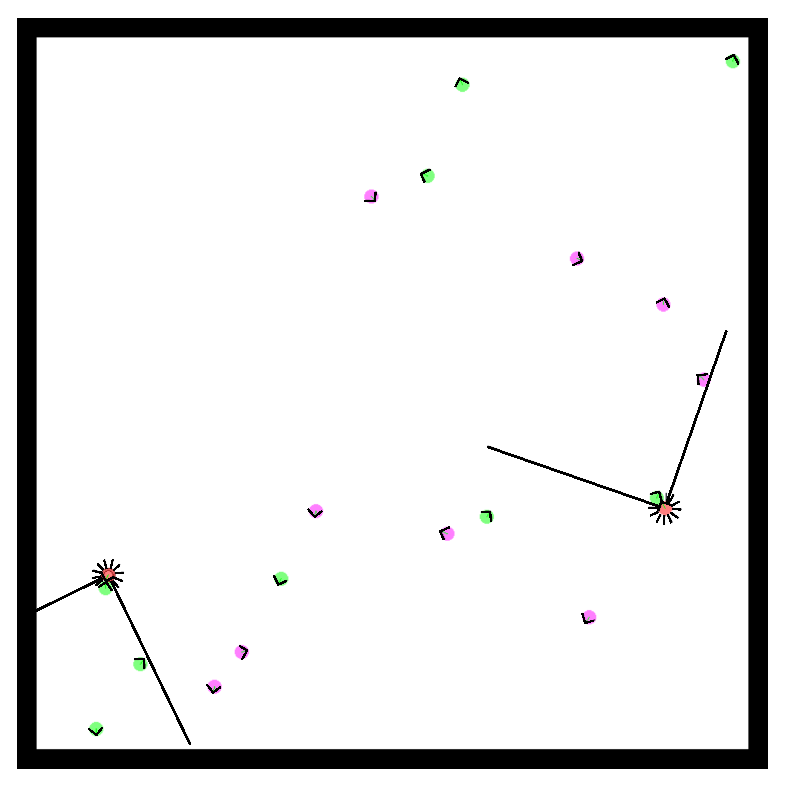
\includegraphics[scale = 0.25]{fig/ArticleBio1/Fig1.eps}
        \caption{\textbf{Screenshot of a robotic simulation.} 
        The red dots represent the two hunters, the green dots the hares, and the pink dots the stags. The black lines around the agents' body represent the proximity sensors and the black cones on front the cameras described in the text. Hunters are allowed to move throughout the environment. Hares and stags remain at their starting positions.}
        \label{fig:figureSimulation}
      \end{figure}

      Food rewards for killing a prey are shown in Table~\ref{table:tableRewardsInitial}. A hare yields a reward of 50, regardless of whether it is hunted in a solitary or cooperative fashion. A stag yields a reward of 500 for each hunter only if it is hunted cooperatively. If a stag is killed by a single hunter, it is still removed from the arena but is considered a failed hunt and rewards nothing. None of the rewards are split between cooperators.

      \begin{table}[ht]
        \centering
          \caption{\textbf{Food rewards for hunting different prey.}}
          \begin{tabular}{|l|r|c|}
            \hline
            \multicolumn{2}{|l|}{\textbf{Prey}} & \textbf{Food Reward} \\
            \hline
            Hare & \textit{alone} & 50 \\
            \hline
            & \textit{coop.} & 50 \\
            \hline
            Stag & \textit{alone} & 0 \\
            \hline
            & \textit{coop.} & 500 \\
            \hline
          \end{tabular}
          \begin{flushleft} The reward depends on whether these prey were hunted alone or cooperatively. There is no reward for stags hunted alone in this case.
          \end{flushleft}
        \label{table:tableRewardsInitial}
      \end{table}

      Simulated robotic agents are evaluated in an 800 by 800 unit square arena, which has four solid walls and is devoid of any obstacles aside from other agents. Each circular-shaped agent, with a diameter of 14 units, is equipped with two independent wheels and a collection of sensors. Hunters can use the information provided by 12 proximity sensors and a front camera. Proximity sensors have a range of approximately twice the diameter of the agent's body, and provide the agent with the proximity of the nearest obstacle. They are evenly distributed around the agent's body. The front camera consists of 12 rays with infinite range spread out in a 90 degree cone in front of the body. Each ray in the camera provides two different pieces of information about the first target it intersects with: the type of target (hunter, hare, or stag) and its proximity. This robot model facilitates the evolution of basic walls avoidance and agents recognition behaviours, which we consider not to be of interest here. Hence we separate obstacles recognition (by the proximity sensors) from agents' recognition (by the camera).

      Only the hunters are capable of movement; prey remain at their initial positions. (Complementary experiments with moving prey capable of avoidance behaviours did not produce significantly different results; not shown.) A prey is caught if any hunter remains close enough during a fixed amount of time steps (800 steps, in a simulation lasting 20.000 time steps). Cooperative hunting is defined as a prey with two hunters in catching distance at the time of its capture. Therefore, cooperation happens even if only one of the two hunters is in catching distance of the prey for most of the time, as long as the two hunters are there in the final step. The prey is then immediately replaced at a random position in the arena, thus keeping a fixed number of agents and prey during the whole simulation.


    \subsubsection{Neural Network for Agent Control}
    \label{nn}
      The hunters' behaviour is computed by an artificial neural network which maps sensory inputs to motor outputs. The neural network is a fully connected multi-layer perceptron with a single hidden layer of 8 neurons. The inputs of this network are the perceptions of the agent, with 12 neurons for the proximity sensors and 48 for the camera (4 for each of the 12 rays) plus a bias neuron (whose value is always 1), for a total of 61 input neurons. The two outputs of the network control the speed of each of the agent's wheels and the mapping function between inputs and outputs is a sigmoid function (see Fig.~\ref{fig:robotDescription}). Changing the number of hidden neurons did not yield significantly different results (not shown).

      \begin{figure}[hbtp]
        \centering
          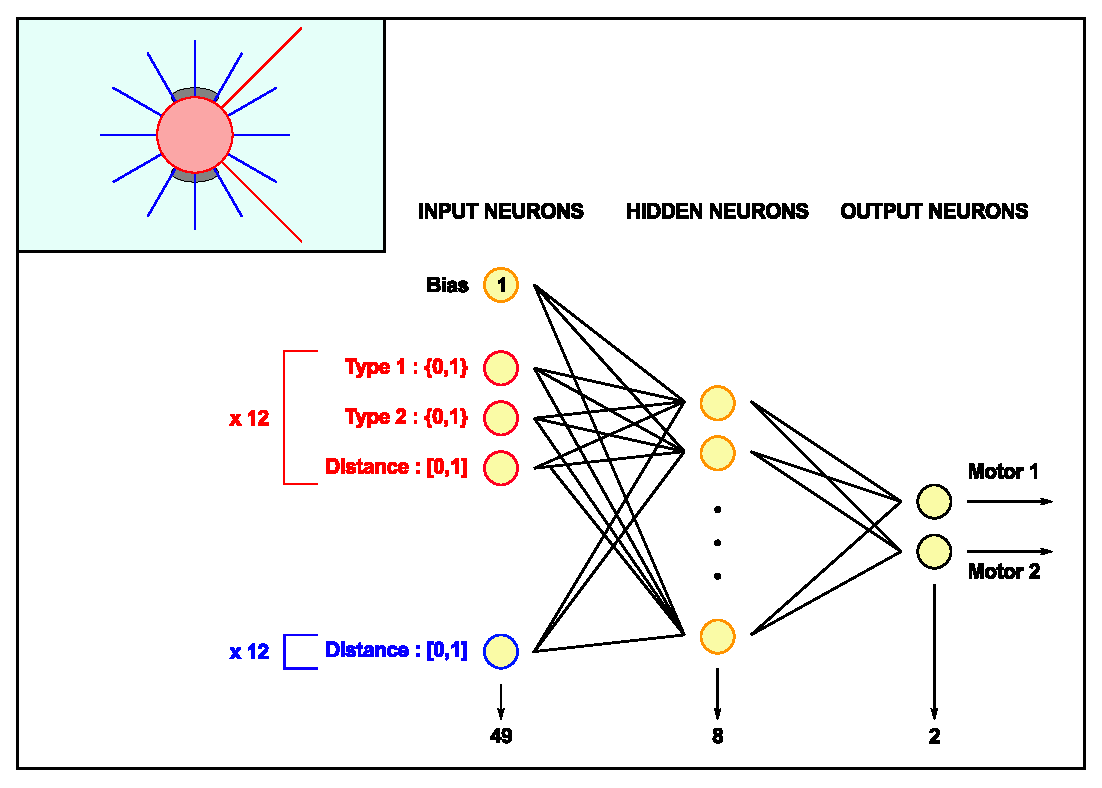
\includegraphics[scale = 0.5]{fig/ArticleBio1/Fig2.eps}
          \caption{\textbf{Diagram of the simulated robotic agent used in the simulation (inset) and its neural network controller.}
          The blue lines represent the 12 proximity sensors and the red lines represent the front camera. Inputs "Type 1" and "Type 2" are two boolean values used to represent the type of the agent (encoded with two bits) recognized by the camera ray.}
        \label{fig:robotDescription}
      \end{figure}


    \subsubsection{Simulating Artificial Evolution} 
    \label{artificialEvolution}
      To simulate evolution, we use an evolutionary algorithm to evolve the genome of the hunters. This genome is comprised of a collection of 410 real values in the range \([0,1]\), one for each of the neural network's weights, and is initially randomized for each individual in the population. In order to obtain its fitness, each individual is successively paired five times with a partner randomly chosen each time (except itself) in the arena presented in the Experimental Setup subsection, for an evaluation round of 20.000 time steps. The payoff of the evaluated individual at the end of a round is given by the total amount of food it has managed to obtain by killing prey in this round. As this quantity depends heavily on the initial conditions (random initial positions of the prey), five simulations are performed for each pair of individuals. The individual's fitness is then obtained by computing the sum of payoffs averaged over the total number of simulations for the individual. In this case the number of simulations is 25, with 5 partners and 5 simulations with each partner.

      Experiments were conducted using a Wright-Fisher model~\cite{Wright1931} with constant population size (20 individuals), which is commonly known as a fitness-proportionate selection method in evolutionary robotics~\cite{Eiben2003}. Using this model, the population of the next generation is formed by a random sampling of offspring from the previous generation, with the probability of sampling a particular parent proportional to the parent's fitness. Each offspring is simply a mutated clone of its parent; recombination is not included in our simulation. Consequently, new genotypes appear only through mutation. These mutations are performed using a Gaussian function, with a standard deviation of \(2 \times 10^{-1}\) and a mutation probability of \(5 \times 10^{-3}\). Each experiment lasted 3000 generations. All simulation parameters are summarised in Table~\ref{table:tableParameters}.

      \begin{table}[ht]
        \centering
          \caption{\textbf{Simulation parameters.}}
          \begin{tabular}{|l|l|c|}
            \hline
            \multicolumn{2}{|l|}{\textbf{Parameter}} & \textbf{Value} \\
            \hline
            \textbf{Evolutionary Algorithm} & & \\
            \hline
            & Selection method & Fitness-proportionate \\
            \hline
            & Population size & 20 \\
            \hline
            & Gene mutation probability & \(5 \times 10^{-3}\) \\
            \hline
            & Mutation operator & Gaussian \(\mathcal{N}(0, 0.01)\) \\
            \hline
            & Number of partners & 5 \\
            \hline
            & Number of simulations per pair & 5 \\
            \hline

            \textbf{Artificial Neural Network} & & \\
            \hline
            & Input neurons & 61 \\
            \hline
            & Hidden neurons & 8 \\
            \hline
            & Output neurons & 2 \\
            \hline
          \end{tabular}
        \label{table:tableParameters}
      \end{table}

  \subsection{Results}
  \label{sec:results}
    \subsubsection{Starting with a population of hare hunters}
      In order to explore the evolutionary transition between the risk-dominant equilibrium (hare hunting) and the payoff-dominant equilibrium (cooperative stag hunting), individuals first evolved in an environment composed solely of hares. This ensured that the populations initially reached the solitary equilibrium. Only then did we add stags and study the dynamics of evolution. Fig.~\ref{fig:hareHuntersRob}(a) shows the evolution of the mean percentage of stags hunted successfully (i.e., hunted cooperatively) out of the total number of prey hunted over time for 30 independent runs. Fig.~\ref{fig:hareHuntersRob}(b) shows the mean proportion of each type of prey hunted during the last generation of each run. Stag hunting evolved in only one run out of $30$ and even in that run accounted for less than 30\% of the total number of prey hunted. In the other $29$ runs, the individuals hunted only hares as they had previously evolved to do. These simulations demonstrate that the evolution of collective hunting is very unlikely when the population is composed of individuals who are already efficient solitary hunters.

      \begin{figure}[hbtp]
        \centering
          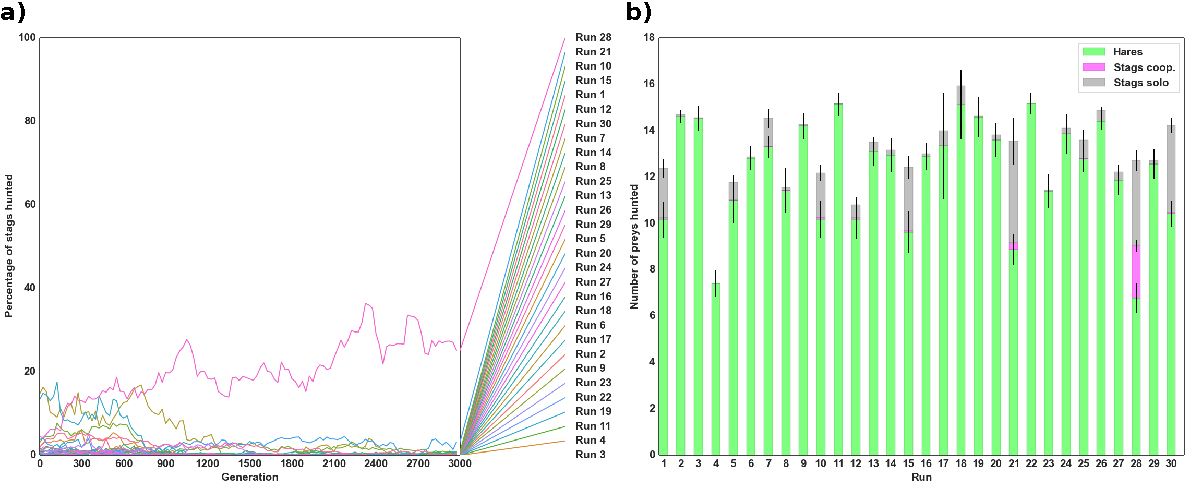
\includegraphics[scale = 1]{fig/ArticleBio1/Fig3.eps}
        \caption{\textbf{Evolution of cooperation in a robotic simulation with an initial hare-hunting strategy.} 
        {\em (a)}~Evolution of the mean percentage of stags hunted successfully (i.e. cooperatively) with respect to the total number of prey hunted. {\em (b)}~Mean number of prey hunted during the last generation of evolution for each independent run. The bottom green bar represents the number of hares hunted, the middle pink bar the number of stags hunted successfully (cooperatively), and the top grey bar the number of failed hunts (stags hunted alone). The standard deviation for each quantity is shown by black lines. The population for each of the 30 independent runs was previously evolved in an environment with only hares. Rewards were 50 for a hare, 0 for a stag hunted alone, and 500 for a stag hunted cooperatively as presented in Table~\ref{table:tableRewardsInitial}. The number of prey ($18$) was kept constant throughout the simulation by replacing killed prey by a prey of the same type.}
        \label{fig:hareHuntersRob}
      \end{figure}

      For comparison we simulated the same scenario using the standard game-theoretic version of the stag hunt, where the expression of the two types of behaviour was encoded by a single binary locus. Each individual in the population initially possessed the allele for hare hunting (Fig.~\ref{fig:hareHuntersTheo}).

      \begin{figure}[hbtp]
        \centering
            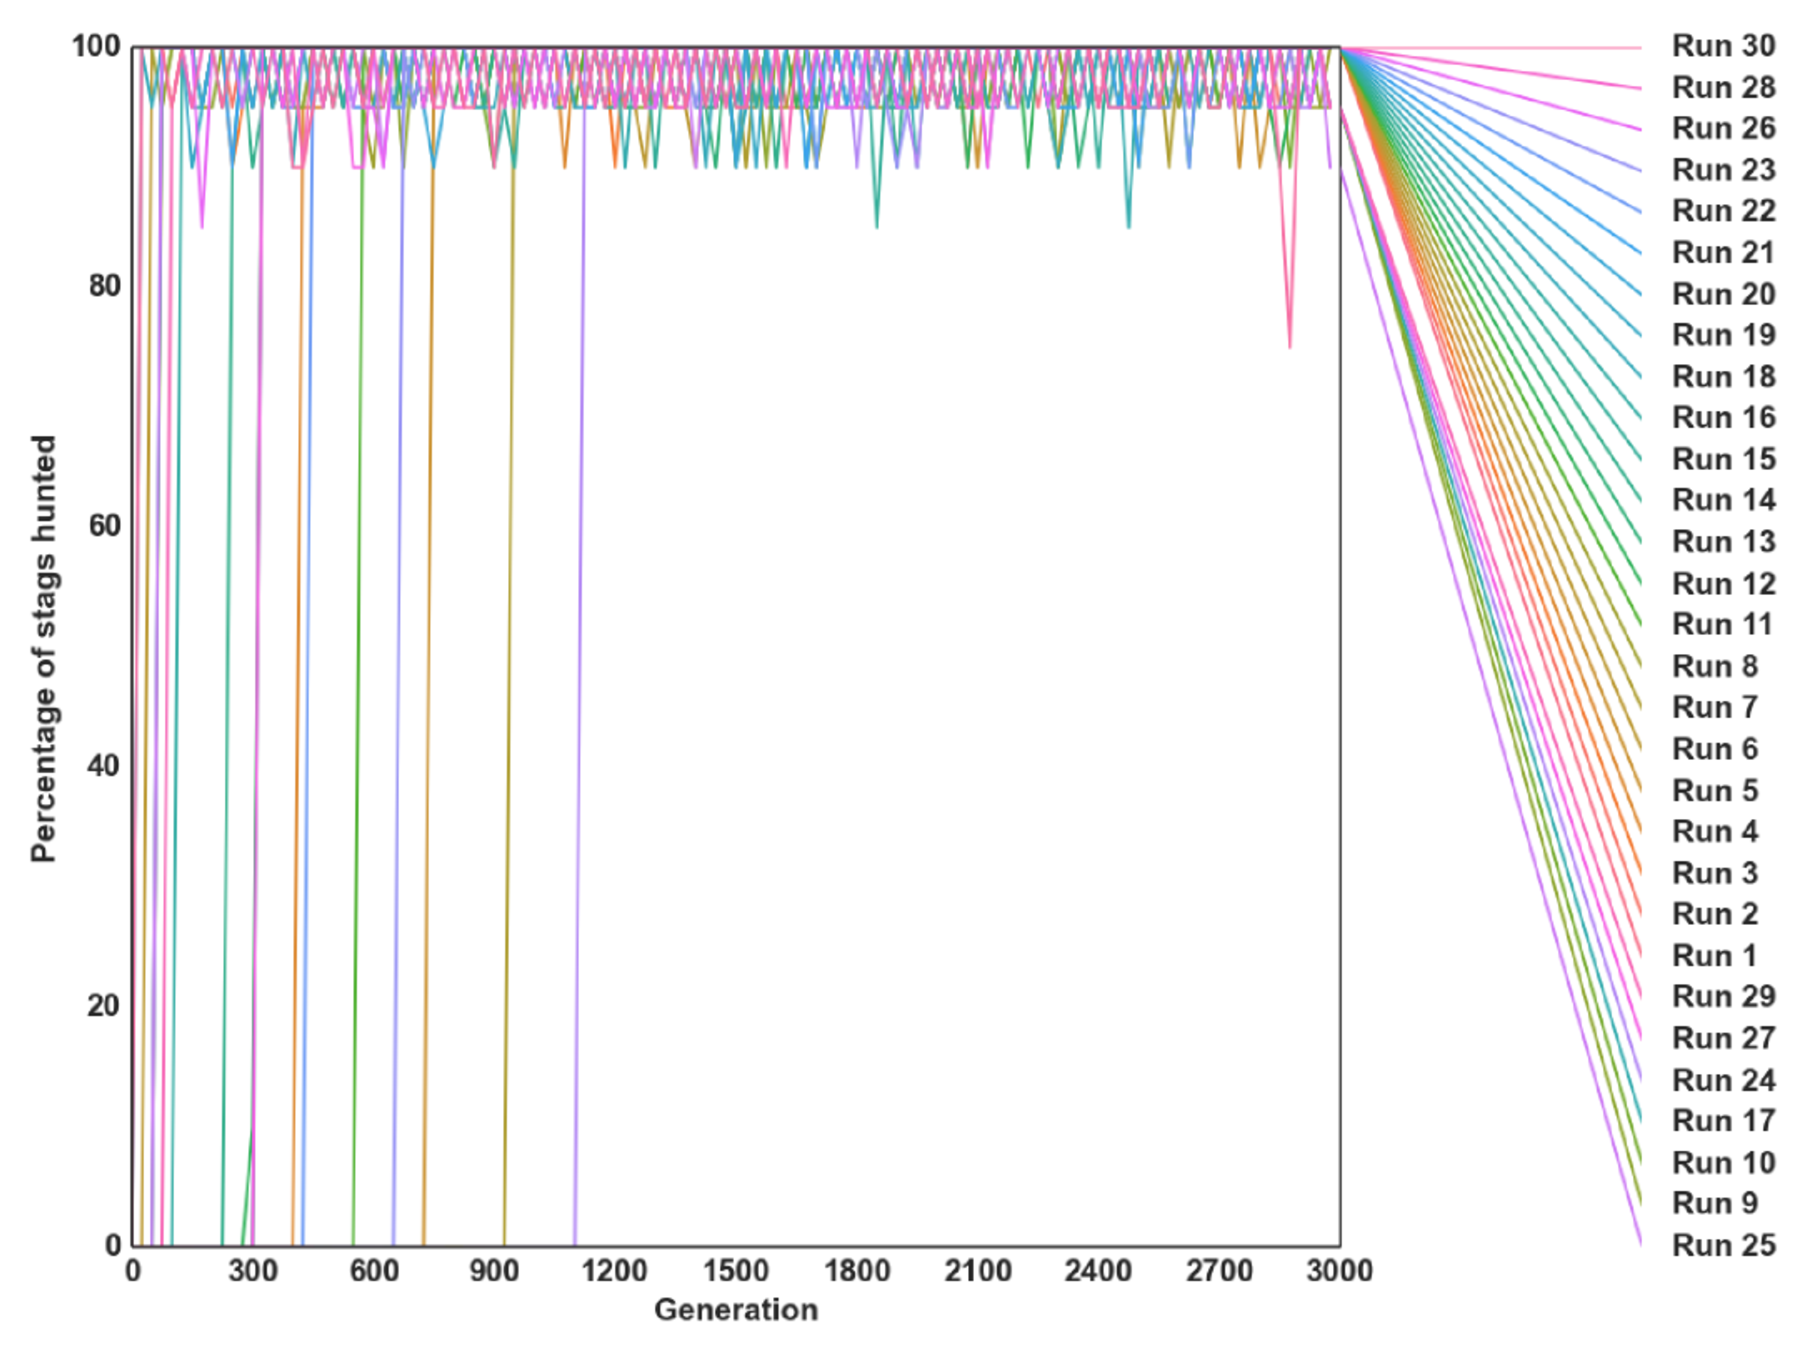
\includegraphics[scale = 0.35]{fig/ArticleBio1/Fig4.eps}
        \caption{\textbf{Evolution of cooperation in a game-theoretic simulation with an initial hare-hunting strategy.} 
        Evolution of the mean percentage of stags hunted successfully (i.e. cooperatively) with respect to the total number of prey hunted when starting with a population of hare hunters for 30 independent runs. Rewards were 50 for a hare, 0 for a stag hunted alone, and 500 for a stag hunted cooperatively as presented in Table~\ref{table:tableRewardsInitial}.}
        \label{fig:hareHuntersTheo}
      \end{figure}

      Here the transition to collective hunting occurred in each of the 30 independent runs and this strategy then remained stable. This result differs drastically from the results of our robotic simulations in which this transition never fully occurred (Mann-Whitney U test on the proportion of stags hunted successfully during the last generation, {\em p}-value \textless 0.001).


    \subsubsection{Starting with a random initial population}
      In a second experiment, we wanted to investigate the evolution of hunting strategies "from scratch", with the individuals' genotypes initialized with random values, rather than evolved with a specific hunting strategy. Fig.~\ref{fig:initialRandom} shows the mean percentage of stags hunted over time and the mean number of prey hunted during the last generation. We observed the transition to a clearly cooperative strategy in a single run, while in two other runs, 50\% of prey hunted were stags. In the $27$ remaining runs the proportion of stags hunted was less than 25\%. In comparison, in simulations using the standard game-theoretic version of the stag hunt where individuals are initially unable to hunt, stag hunting evolved and remained stable in every run (see supporting information, Fig.~\nameref{S1_Fig}).

      \begin{figure}[hbtp]
        \centering
          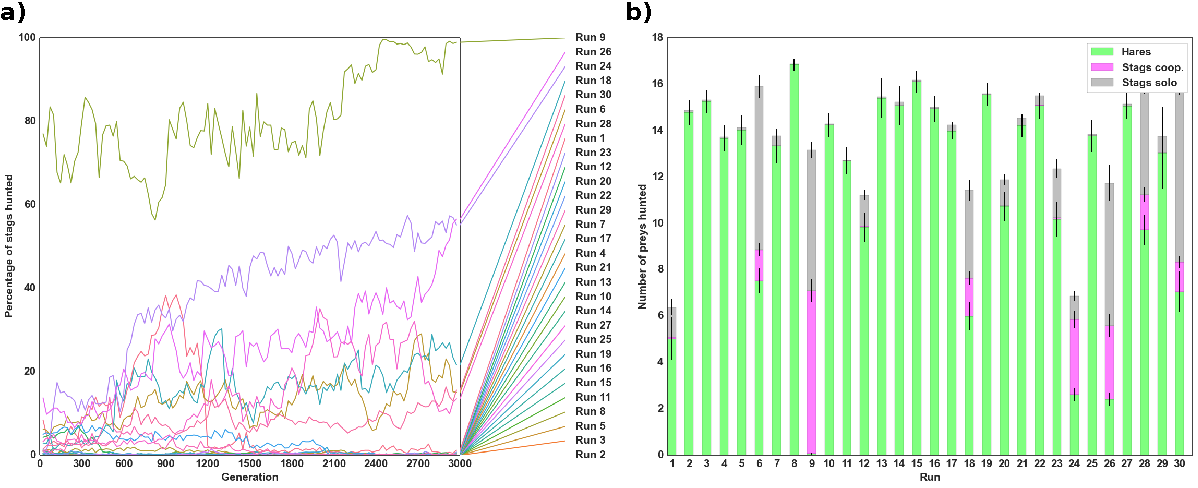
\includegraphics[scale = 1]{fig/ArticleBio1/Fig5.eps}
        \caption{\textbf{Evolution of cooperation with no initial hunting strategy.} 
        {\em (a)}~Evolution of the mean percentage of stags hunted successfully (i.e. cooperatively) with respect to the total number of prey hunted in a robotic simulation. {\em (b)}~ Mean number of prey hunted during the last generation of evolution for each independent run. The bottom green bar represents the number of hares hunted, the middle pink bar the number of stags hunted successfully (cooperatively) and the top grey bar the number of failed hunts (stags hunted alone). The standard deviation for each quantity is shown by black lines. Rewards were 50 for a hare, 0 for a stag hunted alone, and 500 for a stag hunted cooperatively, as presented in Table~\ref{table:tableRewardsInitial}. The number of prey ($18$) was kept constant throughout the simulation by replacing killed prey by a prey of the same type.}
        \label{fig:initialRandom}
      \end{figure}

      The above experiments show that mechanistic constraints have a critical effect on the evolution of coordinated collective actions. In a simple game-theoretic analysis in which the hunting strategy is encoded by a single binary gene, collective behaviour systematically evolved. However, in a setting where the hunting strategy was determined by a more complex artificial neural network, cooperative behaviour evolved in fewer than 10\% of cases. These results encourage further exploration into the evolutionary origin of coordinated collective actions and the mechanisms which may facilitate their evolution. In the following section, we explore two such mechanisms.


    \subsubsection{When stags can be hunted alone}
    \label{successfulCooperation}
      In the next experiment, food was also rewarded for hunting a stag in a solitary fashion so that cooperative behaviour did not entail a risk. We wanted to study whether hunting a stag alone could act as a transition towards the evolution of the collective strategy. Hunting a stag alone was given the same reward as hunting a hare (Table~\ref{table:tableRewardsStagAlone}), differing from classical models of the stag hunt.

      \begin{table}[ht]
        \centering
          \caption{\textbf{Food rewards for hunting different prey.}}
          \begin{tabular}{|l|r|c|}
            \hline
            \multicolumn{2}{|l|}{\textbf{Prey}} & \textbf{Food Reward} \\
            \hline
            Hare & \textit{alone} & 50 \\
            \hline
            & \textit{coop.} & 50 \\
            \hline
            Stag & \textit{alone} & 50 \\
            \hline
            & \textit{coop.} & 500 \\
            \hline
          \end{tabular}
          \begin{flushleft} The reward depends on whether these prey were hunted alone or cooperatively. There is a reward for stags hunted alone in this case.
          \end{flushleft}
        \label{table:tableRewardsStagAlone}
      \end{table}

      Fig.~\ref{fig:graphSolo} shows the results of robotic simulations where individuals initially evolved to hunt hares (as in Fig.~\ref{fig:hareHuntersRob}). As expected, the evolution of collective hunting was significantly facilitated when the risk of hunting stags alone was removed (Mann-Whitney, {\em p}-value \textless 0.001). The populations completely switched to hunting stags in two runs out of 30, and in three other runs, more than 50\% of the prey hunted were stags, with a large part of the prey hunted cooperatively in each of these runs. However, in most of the runs (25 out of 30), the evolved strategy was to hunt both types of prey in a solitary fashion. From these results, it entails that the individuals are still hindered by the evolution of a successful coordination strategy.
      
      \begin{figure}[hbtp]
        \centering
          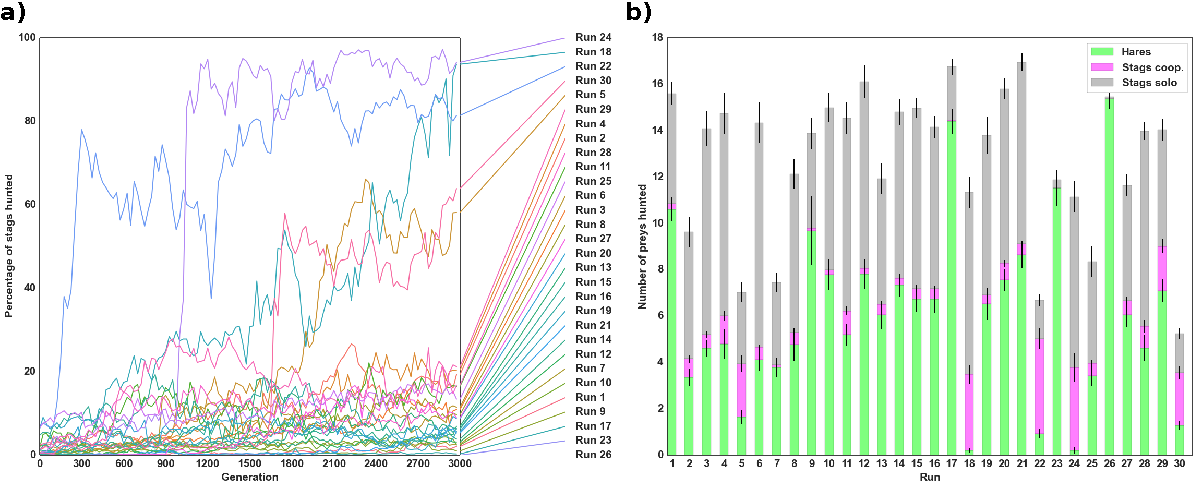
\includegraphics[scale = 1]{fig/ArticleBio1/Fig6.eps}
        \caption{\textbf{Evolution of cooperation with an initial hare-hunting strategy and a reward for solitary stag hunting.}
        {\em (a)}~ Evolution of the mean percentage of stags hunted successfully (i.e. cooperatively) with respect to the total number of prey hunted in a robotic simulation. {\em (b)}~ Mean number of prey hunted during the last generation of evolution for each independent run. The bottom green bar represents the number of hares hunted, the middle pink bar the number of stags hunted cooperatively and the top grey bar the number of stags hunted alone. The standard deviation for each quantity is shown by black lines. The population for each of the 30 independent runs was previously evolved in an environment with only hares. Rewards were 50 for a hare, 50 for a stag hunted alone, and 500 for a stag hunted cooperatively as presented in Table~\ref{table:tableRewardsStagAlone}. The number of prey ($18$) was kept constant throughout the simulation by replacing killed prey by a prey of the same type.}
        \label{fig:graphSolo}
      \end{figure}


    \subsubsection{The role of genetic relatedness}
      Genetic relatedness among social partners is known to influence the evolution of many types of social traits~\cite{Hamilton1964}. In particular,~\cite{Skyrms2004} showed how it can facilitate the evolution of cooperation in a stag hunt game~\cite[chapter 3]{Skyrms2004}. It can yield more frequent interaction between cooperators, which in turn increases their probability of benefiting from cooperative behaviour. In order to include this mechanism, we considered an extreme situation in which each individual is always paired with a clone of itself, known as "clonal selection" in robotics, ensuring a maximal genetic relatedness of 1.

      These results show that genetic relatedness has a positive effect on the evolution of cooperation (Fig.~\ref{fig:graphAltruism}). In four out of 30 runs the population evolved the cooperative strategy. Moreover, in two other runs, stags accounted for more than 75\% of prey hunted, as compared to less than 25\% without relatedness (Mann-Whitney, {\em p}-value \textless 0.005). When the initial population was random, rather than only hare hunters (see supporting information, Fig.~\nameref{S2_Fig}), the positive effect of genetic relatedness was also observed in 12 out of 30 runs, where more than 50\% of prey hunted were stags.

      \begin{figure}[hbtp]
        \centering
          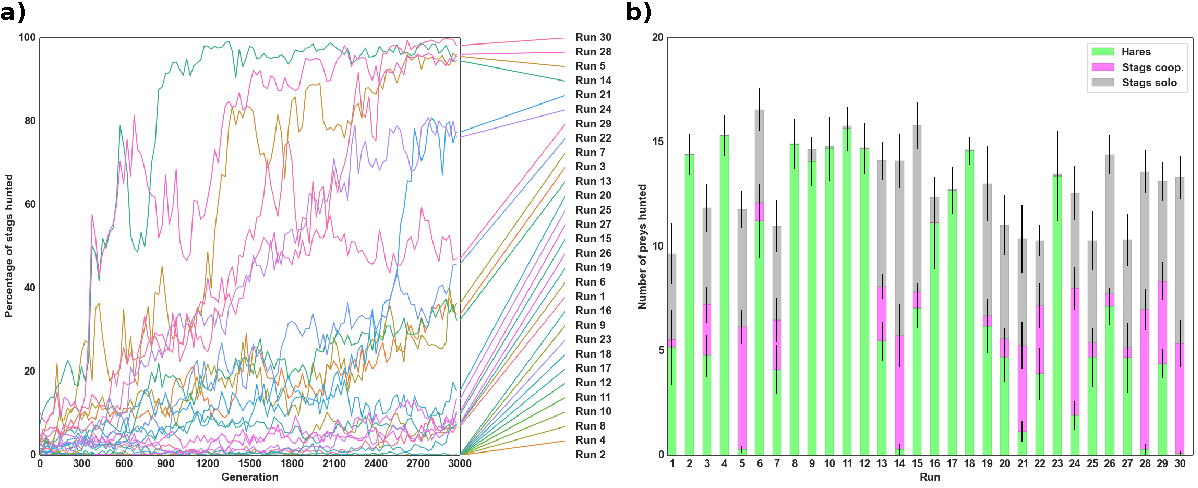
\includegraphics[scale = 1]{fig/ArticleBio1/Fig7.eps}
        \caption{\textbf{Evolution of cooperation under maximal genetic relatedness with an initial hare-hunting strategy.} 
        {\em (a)}~ Evolution of the mean percentage of stags hunted successfully (i.e. cooperatively) with respect to the total number of prey hunted in a robotic simulation. {\em (b)}~ Mean number of prey hunted during the last generation of evolution for each independent run. The bottom green bar represents the number of hares hunted, the middle pink bar the number of stags hunted successfully (cooperatively) and the top grey bar the number of failed hunts (stags hunted alone). The standard deviation for each quantity is shown by black lines. The population for each of the 30 independent runs was previously evolved in an environment with only hares. The genetic relatedness between paired individuals was 1. Rewards were 50 for a hare, 0 for a stag hunted alone, and 500 for a stag hunted cooperatively as presented in Table~\ref{table:tableRewardsInitial}. The number of prey ($18$) was kept constant throughout the simulation by replacing killed prey by a prey of the same type.}
        \label{fig:graphAltruism}
      \end{figure}

  \subsection{Discussion}
  \label{discussion}
    There is a profound difference between evolutionary game-theoretic and robotic simulations of the stag hunt. Using identical model parameters, the transition from the solitary equilibrium to the social equilibrium always occurred in game-theoretic simulations, but was extremely unlikely in robotic simulations, occurring in $1$ run out of $30$. The complexity of the mapping between genotype and phenotype is responsible for much of this contrast. Individuals involved in a coordination game such as the stag hunt face a chicken \& egg problem: the cooperative behaviour must be beneficial in order to evolve, but no individual can benefit from this behaviour unless the behaviour is already expressed by other individuals. When binary variation at a single genetic locus encodes the expression of the solitary or cooperative strategy, a single mutation is sufficient for a cooperative mutant to appear in a resident population of solitary individuals. In a finite population, demographic stochasticity can then lead to the rise of cooperators above the invasion threshold, at which point natural selection leads to their fixation, switching from a solitary equilibrium to a social one. In contrast, in our robotic simulations, the mapping between genotype and phenotype is more complex. Adopting the social strategy entails both a modification of the preferred hunting target and the ability to coordinate with others. Thus, several mutations are necessary for the appearance of full-fledged cooperative behaviour. As several individuals must carry these multiple mutations for the behaviour to become beneficial, the transition to the cooperative equilibrium is nearly impossible.

    In particular, in our robotic simulations we were able to observe that coordination entails a specific and rather complex behaviour. Fig.~\ref{fig:behaviourTraces} (see also supporting information, Movie~\nameref{S1_Movie}) shows the behaviours evolved by the best individuals in the cooperative run shown in Fig.~\ref{fig:initialRandom} (Run $9$). The solution they evolved for coordination was to circle around one another, allowing each of them to constantly see their partner while both moving closer to a stag. This behaviour was replicated in every cooperative run. We thus observed the evolution of an ingenious (given the agents' limited capabilities) and complex hunting strategy. These findings demonstrate that the practical mechanics of behaviour can have important evolutionary consequences, and that models which ignore these properties may lead to misleading predictions.

    Moreover, the evolution of cooperation is also strongly impacted by ecological features. Social hunting poses a bootstrapping problem because it entails both a modification of the preferred hunting target and an ability to coordinate with others. Its evolution can be facilitated, therefore, if hunters have a reasonable probability of hunting the same prey as their partner, just by chance, with no need of active coordination. Biologically, this could occur if hunters live in a dense social environment (with many other hunters in the vicinity), and/or if the density of prey is low, such that the likelihood of ending up on the same prey is large. To test this possibility, we conducted additional experiments where the density of prey was varied. The number of prey was whether (1) decreased from $18$ to $6$ or (2) increased from $18$ to $30$. The population was initially constituted of hare hunters and we kept the same ratio of prey as in previous experiments (i.e. 50\% of hares and 50\% of stags). We show (see supporting information, Fig.~\nameref{S3_Fig}(a)) that when the number of prey is decreased ($6$) the transition to a cooperative strategy is facilitated (Mann-Whitney, {\em p}-value \textless 0.05) as in $9$ runs out of $30$, more than $30$\% of the prey hunted are stags. In comparison, a higher density of prey ($30$) entails that it is impossible to evolve cooperation (see supporting information, Fig.~\nameref{S3_Fig}(b)). These results reinforce our claim that the practical mechanics of coordination are crucial in understanding the evolution of cooperation. In particular, here, the precise ecological situation faced by individuals plays a key role in the transition to the collective equilibrium.

    Finally, the complexity of coordination suggests that the recycling of a previously evolved trait could be necessary for the transition to cooperation, i.e. individuals could coordinate thanks to behavioural features that may not have been selected for cooperation at first. Such features could include the evolution of communication, or a leader-follower strategy. The role of both of these behaviours has already been studied in real-life stag hunt type interactions in chimpanzees and human children~\cite{Bullinger2011, Duguid2014}, and there is an already extensive literature in evolutionary robotics on their role in the evolution of collective actions~\cite{Trianni2007, Mitri2009, Solomon2012, Ferrante2015}. This offers some directions for future works on this problem.


    \begin{figure}[hbtp]
      \centering
        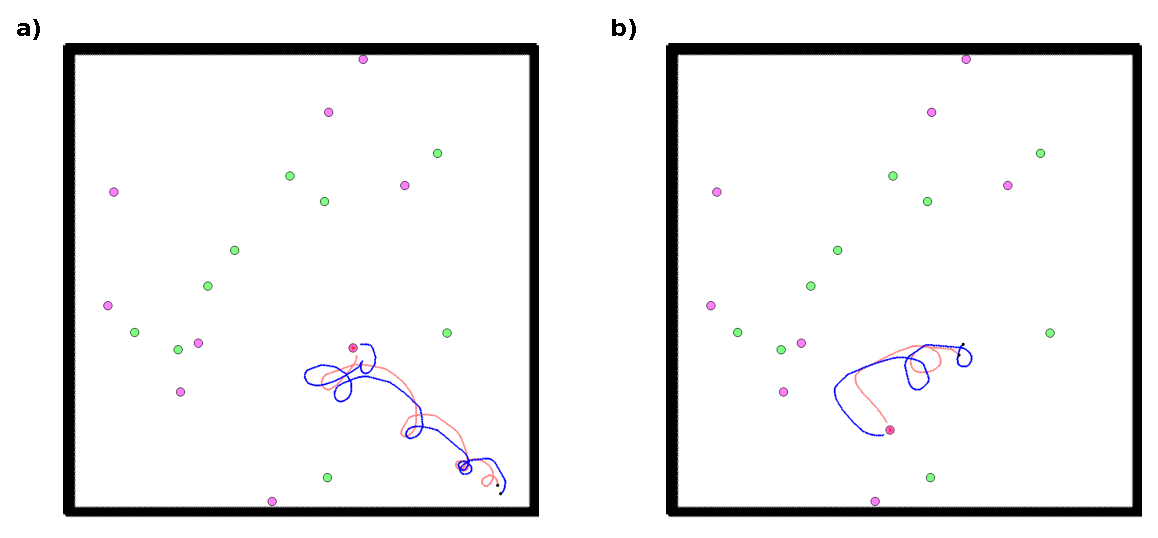
\includegraphics[scale = 1]{fig/ArticleBio1/Fig8.eps}
      \caption{\textbf{Snapshots of a simulation after two hunts.}
      In each of these snapshots, we show the path travelled by each hunter (in different colours) since their last prey was hunted. The black dots represent the positions of the hunters at their last kill. The red star on the stag (pink circle) converged on by the hunters indicates not only that the prey was killed but, more importantly, that it was killed cooperatively by the two hunters.}
      \label{fig:behaviourTraces}
    \end{figure}


  \subsection{Supporting Information}
    \begin{figure}[hbtp]
      \centering
        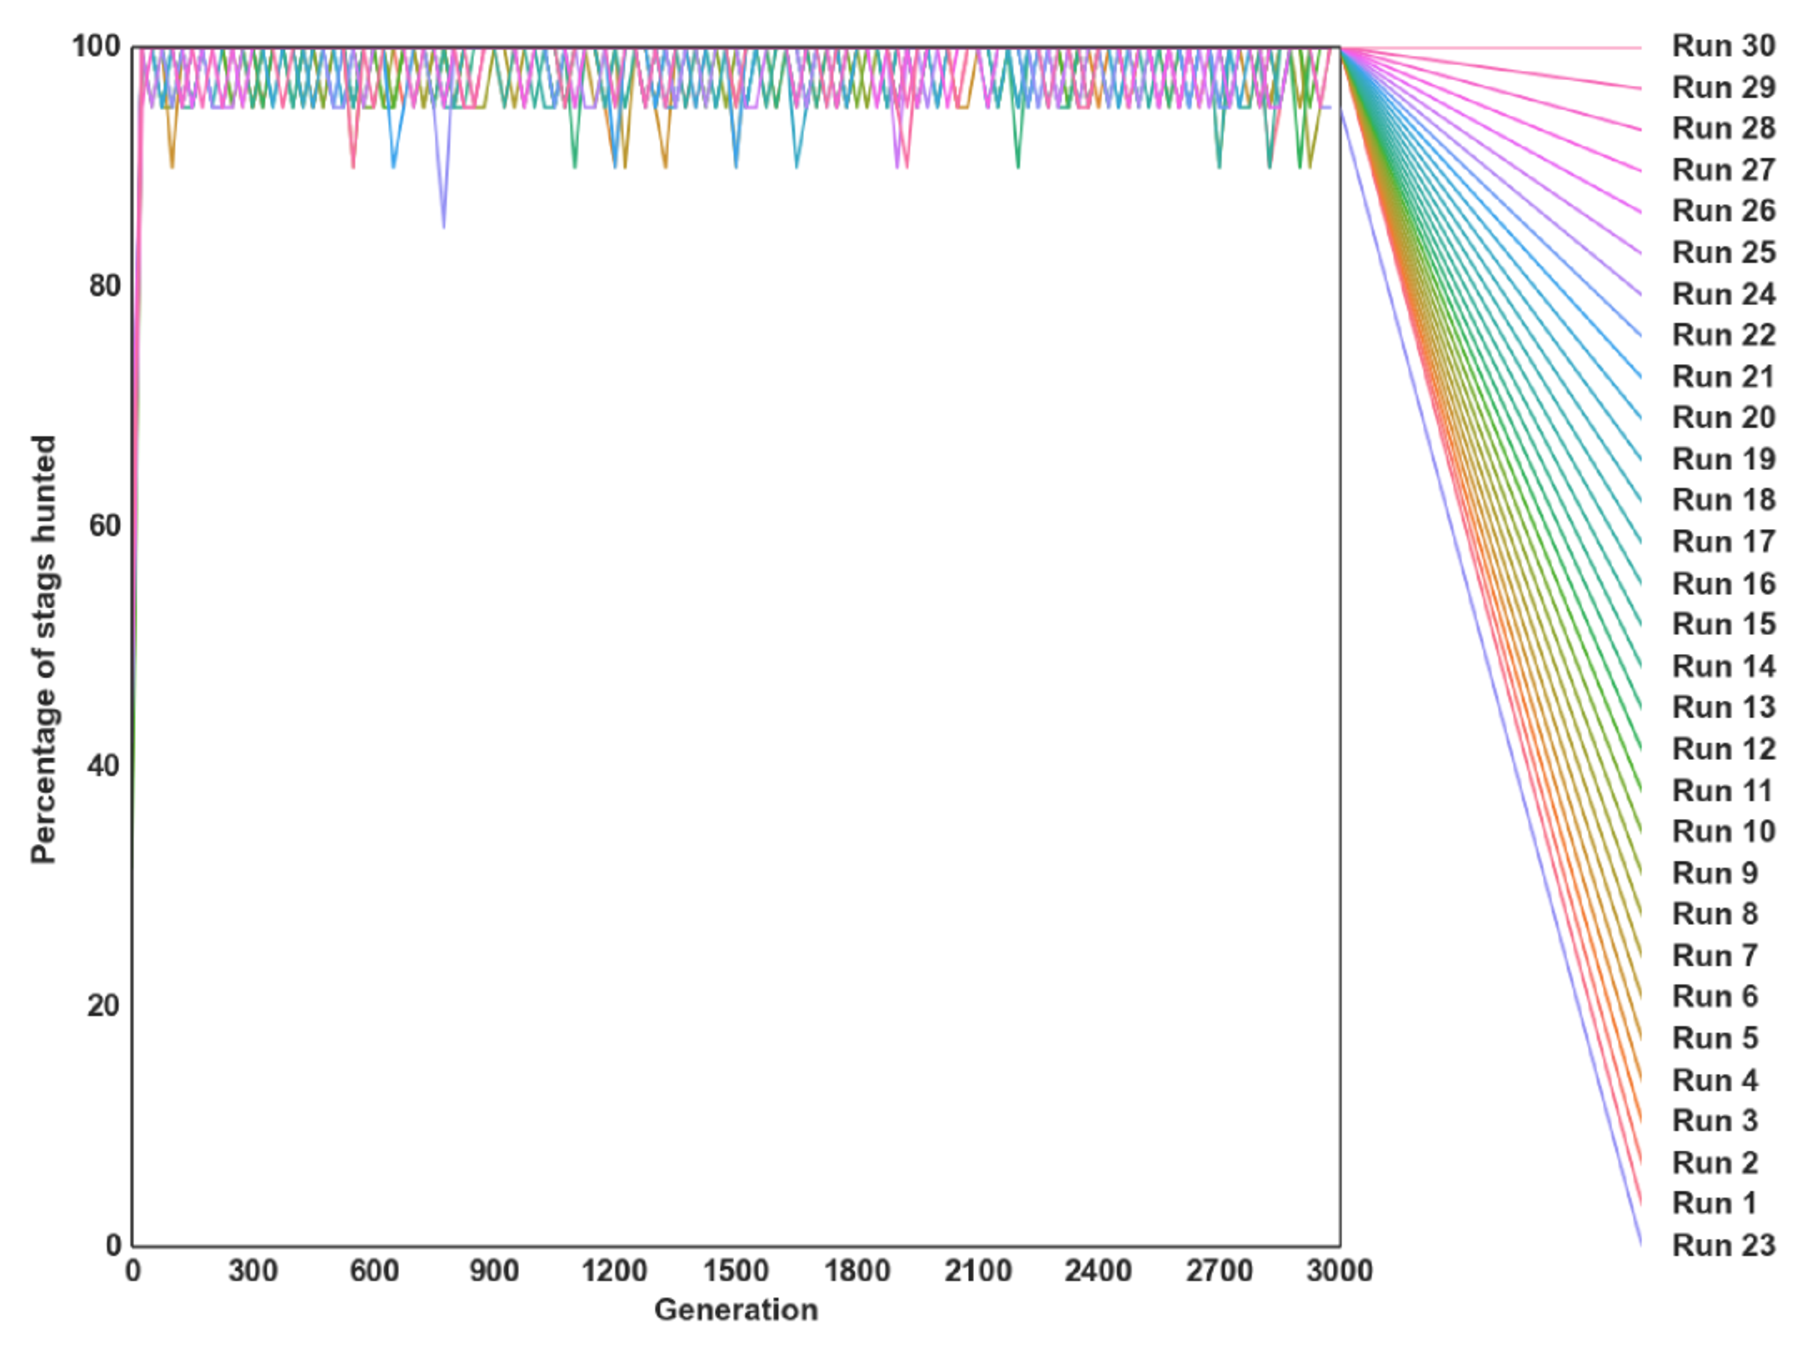
\includegraphics[scale = 1]{fig/ArticleBio1/S1_Fig.eps}
      \caption{\textbf{Evolution of cooperation in a game-theoretic simulation with an initial hare-hunting strategy.} 
      Evolution of the mean percentage of stags hunted with respect to the total number of prey hunted where individuals are initially unable to hunt for 30 independent runs. Rewards were 50 for a hare, 0 for a stag hunted alone, and 500 for a stag hunted cooperatively.}
      \label{S1_Fig}
    \end{figure}

    \begin{figure}[hbtp]
      \centering
        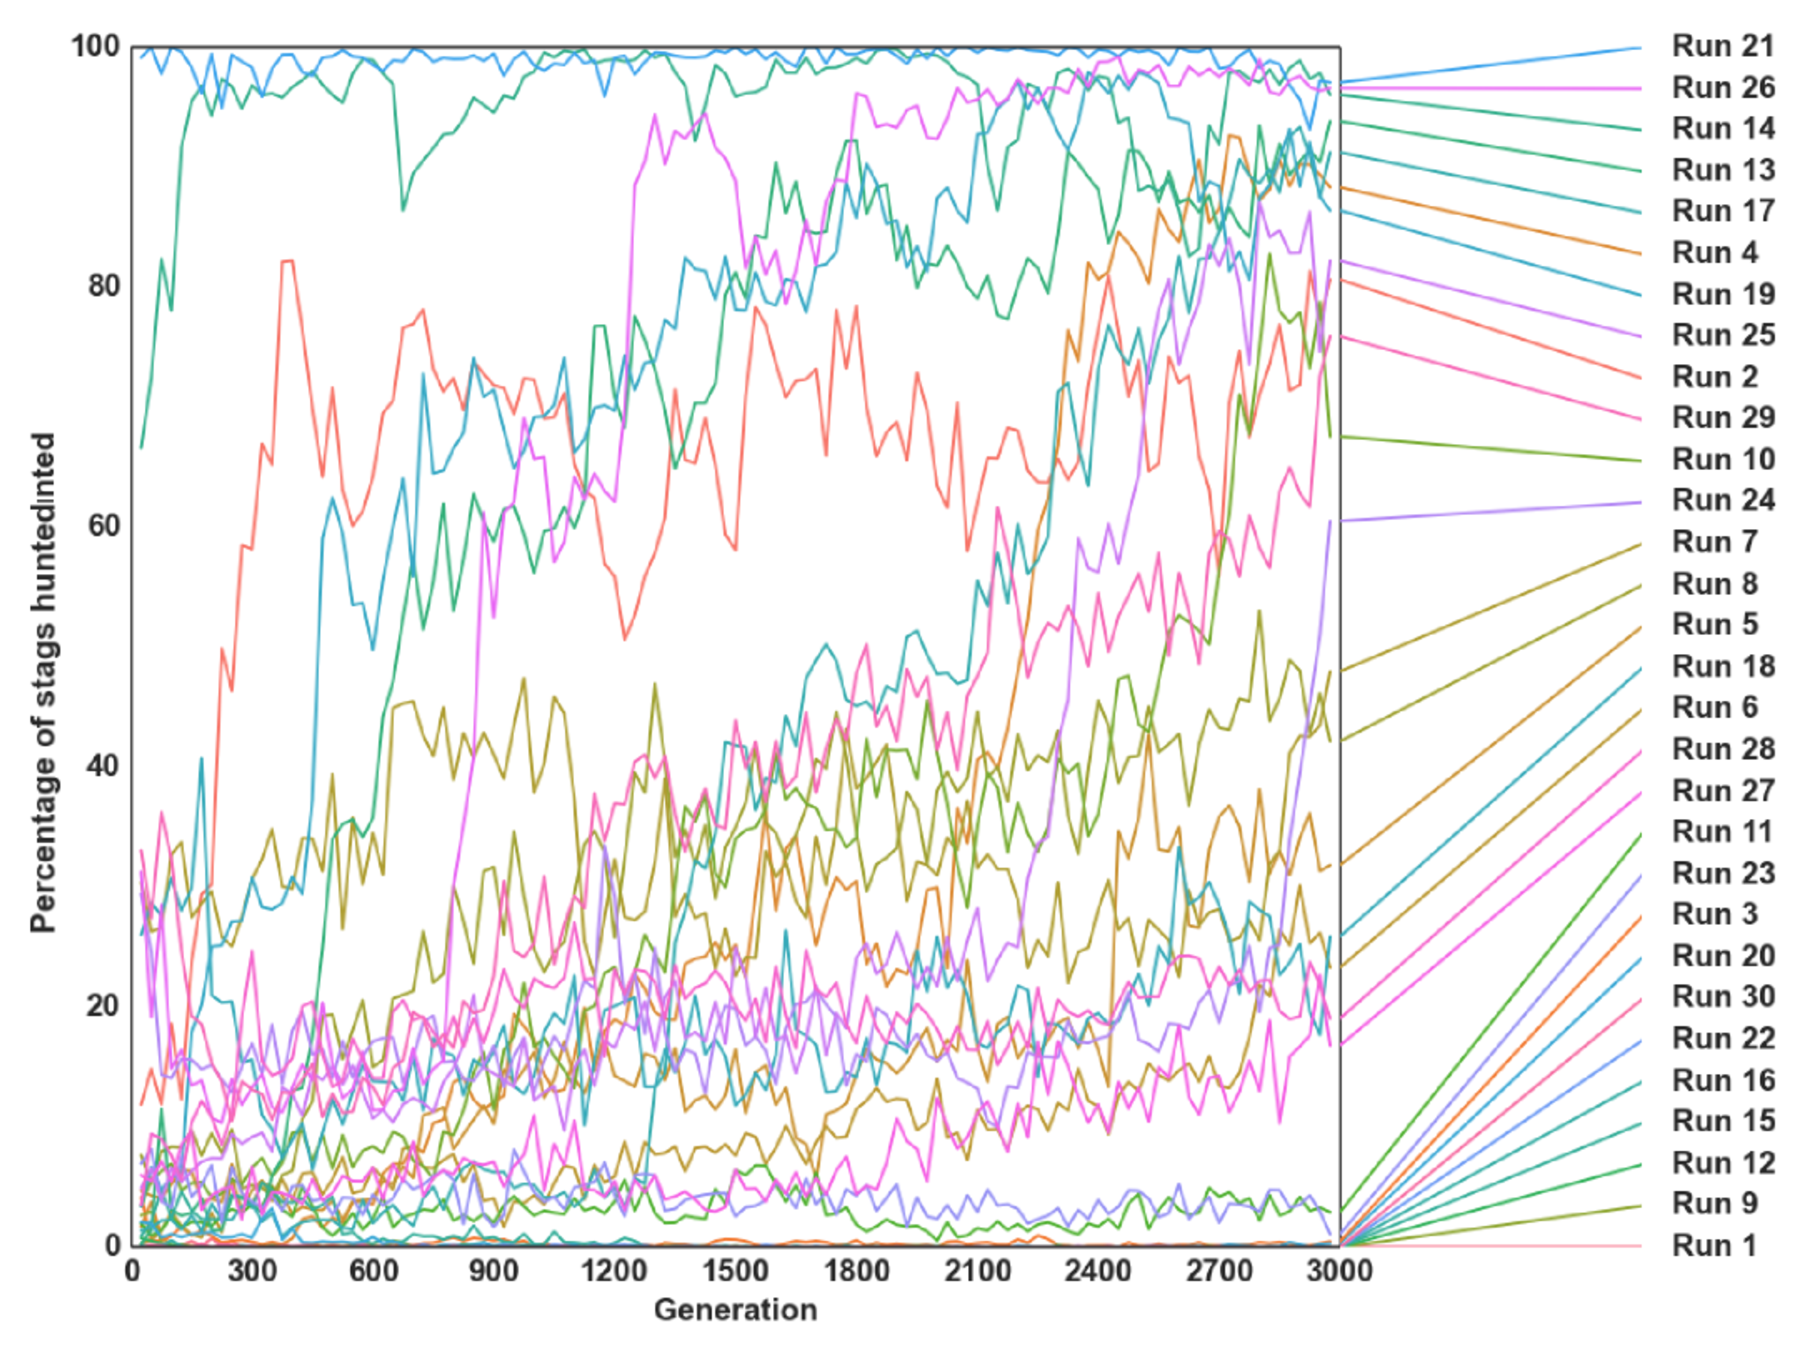
\includegraphics[scale = 1]{fig/ArticleBio1/S2_Fig.eps}
      \caption{\textbf{Evolution of cooperation under maximal genetic relatedness with no initial hunting strategy.}
      Evolution of the mean percentage of stags hunted with respect to the total number of prey hunted in a robotic simulation. The genetic relatedness between paired individuals was 1. Rewards were 50 for a hare, 0 for a stag hunted alone, and 500 for a stag hunted cooperatively as presented.}
      \label{S2_Fig}
    \end{figure}

    \begin{figure}[hbtp]
      \centering
        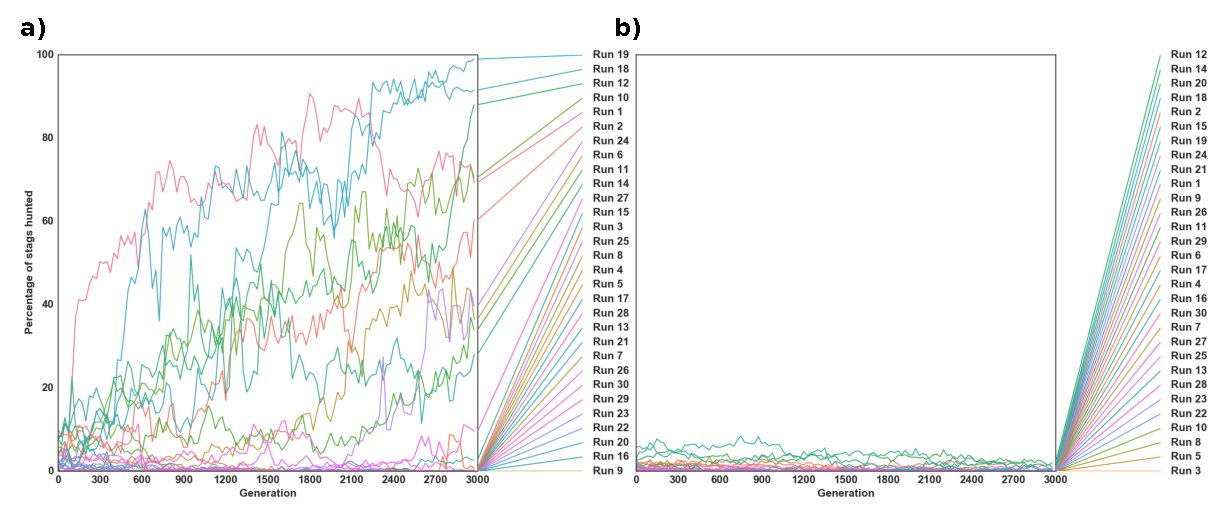
\includegraphics[scale = 1]{fig/ArticleBio1/S3_Fig.eps}
      \caption{\textbf{Evolution of cooperation with an initial hare-hunting strategy and a varied density of prey.} 
      Evolution of the mean percentage of stags hunted successfully (i.e. cooperatively) with respect to the total number of prey hunted in a robotic simulation when the number of prey was {\em (a)} $6$ and {\em (b)} $30$. The population for each of the 30 independent runs was previously evolved in an environment with only hares. Rewards were 50 for a hare, 0 for a stag hunted alone, and 500 for a stag hunted cooperatively as presented in Table~\ref{table:tableRewardsInitial}. The number of prey was kept constant throughout the simulation by replacing killed prey by a prey of the same type.}
      \label{S3_Fig}
    \end{figure}


\section{Article 2}
